




\section{Acceptability study}

In the literature of SA in Turkish it is claimed that SA is only operational for inflectional suffixes \citep{orgun1995flat,kornfilt1996some,broadwell2008turkish, kornfilt2012revisiting} with the exception of \cite{akkucs2016suspended}. Although isolated examples for SA of derivational suffixes can be found in corpora, the literature seems to be treating them as exceptions. One similarity of this exceptionalism can be argued for the instances of SA in German. The examples provided in German \citep{pounder2006broken} has a "-" character at word endings where the suspended affix should be recovered, and the examples are from written literature sources. This might indicate that SA in German is a script-wise use. A similar reasoning can be made for SA of derivational suffixes in Turkish: They are not a language phenomena, they are script-wise exceptions. One way or another, a quantitative exploration into at least some of the derivational suffixes can be made to see to what degree derivational suffixes are capable of SA. For this purpose I have designed a simple acceptability judgment study.
I have taken a subset of the derivational suffixes that take nominal bases and produce nominals from a list in \cite{goksel2004turkish}. I give the derivation examples for the suffixes in (\ref{derivationalsuffixes}).


\begin{exe}
  \begin{multicols}{2}
    \ex \label{derivationalsuffixes}
    \begin{xlist}
        \ex 
        \gll 
        düş-er-cesine \\ fall-{\Aor}-{\Der} \\
        \glt `as if falling'
        
        \ex 
        \gll 
        yalan-cı \\ lie-{\Der} \\ 
        \glt `liar'
        
        \ex 
        \gll 
        kahve-msi renk \\ coffee-{\Der} colour \\
        \glt `like coffee colour'

        \ex 
        \gll 
        üç-üncü \\ three-{\Der} \\
        \glt `third'
        
\columnbreak

        \ex 
        \gll 
        sorun-lu adam \\ problem-{\Der} man \\
        \glt `troubled man'
        
        \ex 
        \gll 
        düşman-lık \\ enemy-{\Der} \\
        \glt `enmity'
        
        \ex 
        \gll 
        sınır-sız internet \\ limit-{\Der} internet \\
        \glt `limitless internet'
        
        \ex 
        \gll 
        iki-şer \\ two-{\Der} \\
        \glt `two by two'
    \end{xlist}
    \end{multicols}
\end{exe}

The suffixes I have chosen do not have a particular property that could make them suitable candidates for SA. However, I have tried to use some of the observations of \cite{yoon2017lexical} where he suggests, in a phase-based morphological derivation, that some suffixes belong to a different morphological phase and retain their atomic properties even after VI. The morphemes that can retain atomicity and syntatic visibility, he claims, choose category assigned bases and can take part in SA. Among the suffixes I have selected, some show differences in what they take as a base and in their function. In (\ref{suffixesdiffer}) I provide a small description for the unique properties for some of them.

\begin{exe}
\ex \label{suffixesdiffer}
\begin{itemize}
\item \textit{-CasInA} can take bases that are modified with a participle like {\Prf}, {\Prog}, or {\Aor}. 

\item \textit{-CI} takes noun bases and it is an agent nominalizer

\item \textit{-(I)msI} takes adjective bases and returns a degree adjective

\item \textit{-(I)ncI} takes numerals and returns an ordinal numeral

\item \textit{-(ş)Ar} takes numerals and returns adverbs

\end{itemize}
\end{exe}

I have selected SA of {\Acc} as a comparison for the suspendability of the derivational suffixes. I have also included a different conjoiner \textit{veya} "or" for the SA environment since this was already an exploratory study. The additional conjoiner differs in its semantic properties as to what conjunction is finally formed. It can be thought as conjoiner \textit{ve} "and" plus additional calculations of truth conditions and/or contexts. My purpose in this experiment is to investigate how much the SA of the suffixes in (\ref{derivationalsuffixes}) are acceptable and how they compare to SA of {\Acc}. For this purpose I have designed an acceptability study where a simple yes or no answer is provided for an expression hosting an SA construction. In the following subsections I lay out the participants, materials, results, and analysis of the experiment.

\subsection{Participants}

The participants are 214 students from Boğaziçi University who are native speakers of Turkish. In exchange for their participation they have received 1 point to their overall course score.

\subsection{Materials}

The experiment is comprised of 9 different suffixes (8 derivational and 1 inflectional {\Acc}) by 2 conjoiners per suffix. For each suffix there are 3 distinct items. This way there are 54 experimental items. Additionally there are 27 grammatical and 27 ungrammatical fillers. A latin square design by conjoiner type is applied, forming two lists of 27. This resulted in each participant seeing only 27 experimental items and 54 fillers. The order of trials is randomized for each participant. An example set of experimental items for {\Acc} and \textit{-CAsInA} is given in (\ref{acceptabilityexe}).

\begin{exe}
    \ex \label{acceptabilityexe}
    \begin{xlist}
    \ex {\Der}\_{\And} \gll \textit{Ev-e} \textit{koş-ar} \textit{ve} \textit{zıpla-r-casına} \textit{gel-di-m.} \\ house-{\Dat} run-{\Aor} {\And} jump-{\Aor}-{\Der} come-{\Pst}.{\First}.{\Sg} \\
    
    \ex {\Der}\_{\Or} \gll \textit{Ev-e} \textit{koş-ar} \textit{veya} \textit{zıpla-r-casına} \textit{gel-di-m.} \\ house-{\Dat} run-{\Aor} {\Or} jump-{\Aor}-{\Der} come-{\Pst}.{\First}.{\Sg} \\
    \glt `I came home as if running and/or jumping.' 
 
    \ex {\Infl}\_{\And} \gll \textit{Ev-e} \textit{defter} \textit{ve} \textit{kitab-ı} \textit{getir-di-m.} \\ house-{\Dat} notebook {\And} book-{\Acc} bring-{\Pst}.{\First}.{\Sg} \\
    
    \ex {\Infl}\_{\Or} \gll \textit{Ev-e} \textit{defter} \textit{veya} \textit{kitab-ı} \textit{getir-di-m.} \\ house-{\Dat} notebook {\Or} book-{\Acc} bring-{\Pst}.{\First}.{\Sg} \\
    \glt `I brought home the book and/or the notebook.' 
    \end{xlist}
\end{exe}

Pre and post sentence fields are not kept constant since each suffix required a different type and place of modification or use, resulting in uneven number of words. The only measurement of the acceptability study is grammaticality judgements and response times. The experiment is formed using http://spellout.net/ibexfarm/ \citep{drummond2013ibex}, and carried out online. For the full list of items and fillers (1-27 and 100-154), see Appendix \ref{acceptabilityitems}.

\subsection{Procedure}
Participants are provided a link to the experiment prompting them with a consent page. Upon giving consent participants go through 5 practice items and then they are prompted again for the beginning of the experiment. Each item is presented as a full sentence and participants decide on whether or not the sentence they encounter is a natural/ok sentence in Turkish. They profess their decision by pushing "Q" key for "yes" and "P" key for "no" on the keyboard. The experiment only recorded choice and response time. After the experiment is done, participants are redirected to a separate page where they provided their student information to be relayed to the course's professor for the extra credit. This is kept separate of the experiment results, keeping participant information and experimental data anonymous.

\subsection{Results}

The results are recorded onto a csv file and imported to R \citep{team2013r}. They include subject, item number, response and response time for each trial. Categories for suffix and conjoiner type and category for experimental item or filler is added. This resulted in 17415 of data points. 1 item with a typo and 1 item with a possible ambiguity are excluded from the data. A further 3 filler items are excluded because they had particular configurations that lead to increased misparsing like garden path sentences and minor ungrammaticalities. After this exclusion, accuracies of the participants are calculated relying on their answers for filler items. Participants with accuracies lower than 70\% are excluded from the data. Trials that are not between 2 and 7 seconds of response time are considered outliers and also excluded from the data. This cleaning process resulted in the loss of 30\% of the data. In Figure \ref{fig:suffixacceptability} I give the average acceptability of each suffix by conjoiner type\footnote{from here on out all vertical errorbars indicate standard errors.}.

\begin{knitrout}
\definecolor{shadecolor}{rgb}{0.969, 0.969, 0.969}\color{fgcolor}\begin{figure}[hbt!]

{\centering 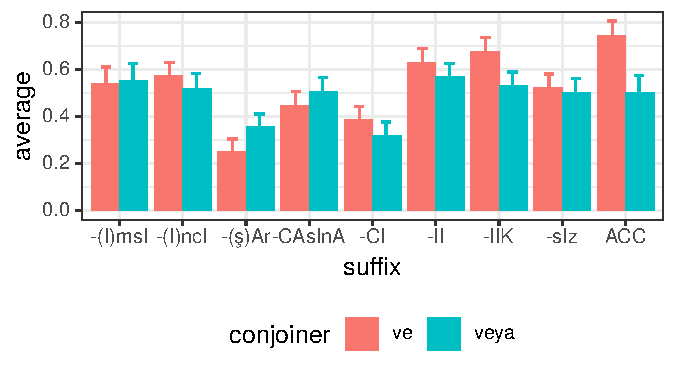
\includegraphics[]{figure/suffixacceptability-1} 

}

\caption[Average acceptability of suffixes by conjoiner]{Average acceptability of suffixes by conjoiner}\label{fig:suffixacceptability}
\end{figure}


\end{knitrout}

Following the mean acceptabilities of each suffix I have fitted a linear mixed model using brms package \citep{burkner2017brms},  conjoiner and suffix type as predictors. I have used sum contrasts for both of the predictors. I also controlled for random effects of item and subject. I give the results of the model in Figure \ref{fig:derivationalmodel}\footnote{points indicate median estimate, bold lines indicate 95\% credible interval and thin lines indicate the whole probability space}. 

\begin{knitrout}
\definecolor{shadecolor}{rgb}{0.969, 0.969, 0.969}\color{fgcolor}\begin{figure}[hbt!]

{\centering 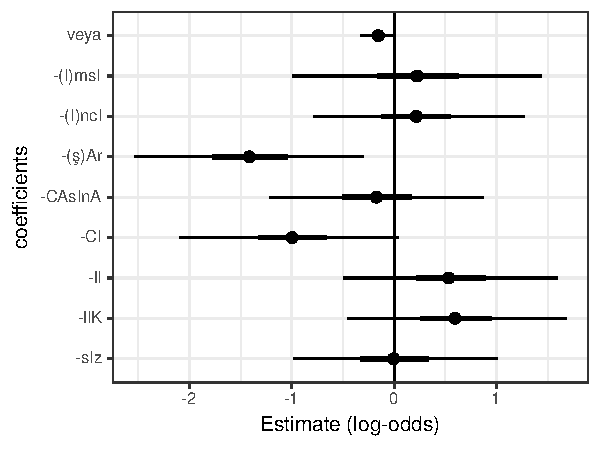
\includegraphics[]{figure/derivationalmodel-1} 

}

\caption[Results of the linear mixed model for derivational suffixes]{Results of the linear mixed model for derivational suffixes}\label{fig:derivationalmodel}
\end{figure}


\end{knitrout}

\subsection{Analysis}

First of all Figure \ref{fig:derivationalmodel} shows that the probability space is much more wider for the derivational suffixes than it is for the intercept. One of the reasons for this is the low item count for each suffix. As expected the probability space for the SA of {\Acc} is packed closer than it is for the derivaitonal suffixes. The conjoiner choice of \textit{veya} "or" also decreases the acceptability for SA of {\Acc}. The estimates that are above 0 with credible intervals not going through 0 mean that they are relatively likely to be acceptable in SA. The estimates that are below 0 with credible intervals not going through 0 mean that they are relatively unlikely to be acceptable in SA. There are also interaction terms indicated with a double column ":" for the coefficients. These levels indicate whether there is a relational effect for the levels of "Suffix" and "conjoiner". These are posterior probabilities and the estimates do not indicate significance. They indicate the probability space for the estimates. It is clear in the results provided in Figure \ref{fig:derivationalmodel} that it is not very likely for the derivational suffixes to be suspended except for the suffixes \textit{-lI} and \textit{-lIK}. There is an interaction between the conjoiner being \textit{veya} "or" and the suffixes \textit{-(ş)Ar} and \textit{-CAsInA}, suggesting a suspendability. However the conjoiner \textit{veya} "or" decreases the acceptability for SA of {\Acc}. This indicates that the interaction terms look like suspendability but compared to SA of {\Acc} they are not suspendable.


The overall interpretation of the average acceptabilities and the model results indicate that SA of derivational suffixes in Turkish do not actually rely on an explanation of morphological phases. The reason for this is that the suffixes \textit{-(ş)Ar, -CAsInA}, and \textit{-(I)msI} take specific bases which are participle forms or belong to specific lexical categories. A possible explanation can be made for the frequencies of the suffixes. For this purpose I have extracted the frequencies of the four derivational suffixes \textit{-lI,-lIK,-sIz}, and \textit{-CI} from TS Corpus \citep{sezer2013ts}. I give the relative proportion of the suffixes in Figure \ref{fig:suffixcorpus}.


\begin{knitrout}
\definecolor{shadecolor}{rgb}{0.969, 0.969, 0.969}\color{fgcolor}\begin{figure}[hbt!]

{\centering 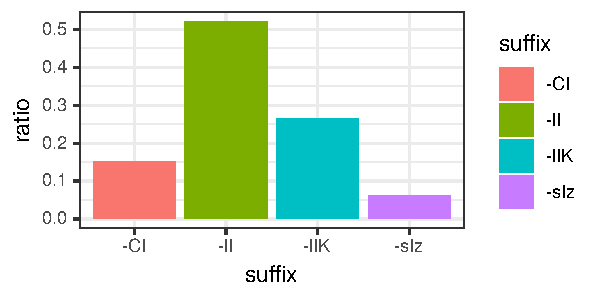
\includegraphics[]{figure/suffixcorpus-1} 

}

\caption[Relative proportion of derivational suffixes in TS Corpus]{Relative proportion of derivational suffixes in TS Corpus}\label{fig:suffixcorpus}
\end{figure}


\end{knitrout}

It is clear that the suffixes that might be suspended are the ones that are the most frequent out of the four even though the proportions of the suffixes are not similarly reflected in the experiment results. Unfortunately not all derivational suffixes of Turkish are represented in corpus data. I have only taken the ones that were included in my expreriment and in the corpus. A further support for the script-wise nature of the SA of derivational suffixes can come from the corpus searches. For example there are plenty of hits for SA of \textit{-(I)ncI} in corpus data. In (\ref{tsinciquerry}) I provide two small CQP searches \citep{hardie2012cqpweb} for SA of \textit{-(I)ncI}, for the numbers ranging from one to five, and for \textit{-(I)msI} with adjective bases. 

\begin{exe}
\ex \label{tsinciquerry}
\begin{xlist}
\ex \textit{-(I)ncI} TS corpus search key
\sn {[word="(bir{\textbar}iki{\textbar}üç{\textbar}dört{\textbar}beş)"][word="ve"][word="(.+nc(ı{\textbar}i{\textbar}u{\textbar}ü))"]}

\ex \textit{-(I)msI} TS corpus search key
\sn {[PosTag="Adj"][word="ve"][PosTag="Adj" \& word="(.+ms(ı{\textbar}i{\textbar}u{\textbar}ü))"]}
\end{xlist}
\end{exe}

There are hundreds of hits for the SA of \textit{-(I)ncI} within the first $\sim$1000 hits yet the acceptance rate for the SA of it is around $\sim$50\% as the Figure \ref{fig:suffixacceptability} shows. The same can not be said for the SA of \textit{-(I)msI} which also has the same acceptance rate as \textit{-(I)ncI} but the corpus search does not result in an SA of \textit{-(I)msI} within the first $\sim$1000 hits. I take this contrast in corpus search and similar acceptance rates in the experiment as an indication for the script-wise nature of the SA of derivational suffixes. Examples regarding them can be found in corpus yet the isolated acceptance rates are lower than of {\Acc}. This indicates that the SA of derivational suffixes are tabloid or literacy choices made for script-wise reasons. However this suggests that in context provided examples or in normal language use where people are not subjected to grammaticality choice, the SA of derivational suffixes might become marginally acceptable. As a result this experiment showed that the acceptability for SA of the derivational suffixes does not particularly follow from a structural interpretation of the derivational suffixes. It might be based on frequency of the suffixes or the specific environments where SA is knowingly made.










